% !TeX root = ../main.tex
\section{Исследование интермодуляционных искажений третьего порядка и определение точки пересечения ($IP_3$)}

\subsection{Теоретические сведения и методика проведения измерений}

При одновременной подаче на вход нелинейного усилителя двух гармонических сигналов с близкими частотами $f_1$ и $f_2$ на выходе, помимо усиленных основных тонов, образуются комбинационные составляющие высших порядков. Наибольшую опасность для радиотракта представляют интермодуляционные составляющие 3-го порядка на частотах $2f_1 - f_2$ и $2f_2 - f_1$, поскольку они попадают в непосредственную близость к полезному сигналу и не могут быть отфильтрованы линейными селективными цепями.

Характеристикой нелинейности по интермодуляции служит \textbf{точка пересечения третьего порядка} ($IP_3$ --- \textit{Third-Order Intercept Point}). Это расчетная точка, в которой экстраполированная малосигнальная линейная зависимость мощности полезного сигнала (наклон 1:1) пересекается с экстраполированной зависимостью мощности продуктов интермодуляции 3-го порядка (наклон 3:1).

\textbf{Основные расчетные соотношения:}
\begin{itemize}
    \item Относительное подавление интермодуляционных составляющих 3-го порядка:
    \begin{equation}
    IMD_3\,[\text{дБ}] = P_{f_{1,2}} - IM_3,
    \end{equation}
    где $P_{f_{1,2}}$ --- мощность основного тона на выходе усилителя, $IM_3$ --- мощность продукта интермодуляции ($2f_1 - f_2$ или $2f_2 - f_1$).
    \item Точка пересечения по выходу ($OIP_3$):
    \begin{equation}
    OIP_3\,[\text{дБм}] = P_{f_{1,2}} + \frac{IMD_3}{2}.
    \end{equation}
    \item Точка пересечения по входу ($IIP_3$):
    \begin{equation}
    IIP_3\,[\text{дБм}] = OIP_3 - K_p,
    \end{equation}
    где $K_p$ --- малосигнальный коэффициент передачи измерительного тракта в децибелах.
\end{itemize}

\textbf{Порядок выполнения эксперимента:}
\begin{enumerate}
    \item Собрана схема формирования двухтонового испытательного сигнала (рис.~29 методических указаний). Сигналы от двух генераторов Advantex SG8 с разницей частот $\Delta f = 1\text{ МГц}$ ($f_1 = 999.0\text{ МГц}$, $f_2 = 1000.0\text{ МГц}$) через развязывающие аттенюаторы 20~дБ поданы на входы сумматора мощности (Power Combiner 1:2).
    \item Двухтоновый сигнал через согласующий аттенюатор 10~дБ подан на вход исследуемого усилителя. Выход усилителя соединен со входом анализатора спектра RIGOL DSA1030 через защитный аттенюатор 6~дБ и Кабель 3].
    \item На анализаторе спектра установлена центральная частота $f_0 = 1.0\text{ ГГц}$, полоса обзора $\text{Span} = 10\text{ МГц}$, полоса пропускания фильтра ПЧ $\text{RBW} = 100\text{ кГц}$, полоса видеофильтра $\text{VBW} = 100\text{ Гц}$ для подавления шумовых флуктуаций дорожки.
    \item Изменяя мощность генераторов $P_{\text{вх}}$ в диапазоне от 0 до $+10\text{ дБм}$, с помощью функции дельта-маркера (`Marker Delta`) анализатора спектра измерены уровни мощности основных тонов $P_{f_{1,2}}$, продуктов $IM_3$ и величина подавления $IMD_3$.
    \item Выполнена проверка линейности измерительного тракта (рис.~30 методических указаний) для исключения перегрузки смесителя анализатора спектра.
\end{enumerate}

\subsection{Результаты экспериментальных исследований}

На рисунках~\ref{fig:sg_screen}--\ref{fig:rigol_spec2} представлены экран генератора с параметрами испытательного тона и спектрограммы двухтонового сигнала на выходе тракта при различных уровнях мощности.

\begin{figure}[H]
    \centering
    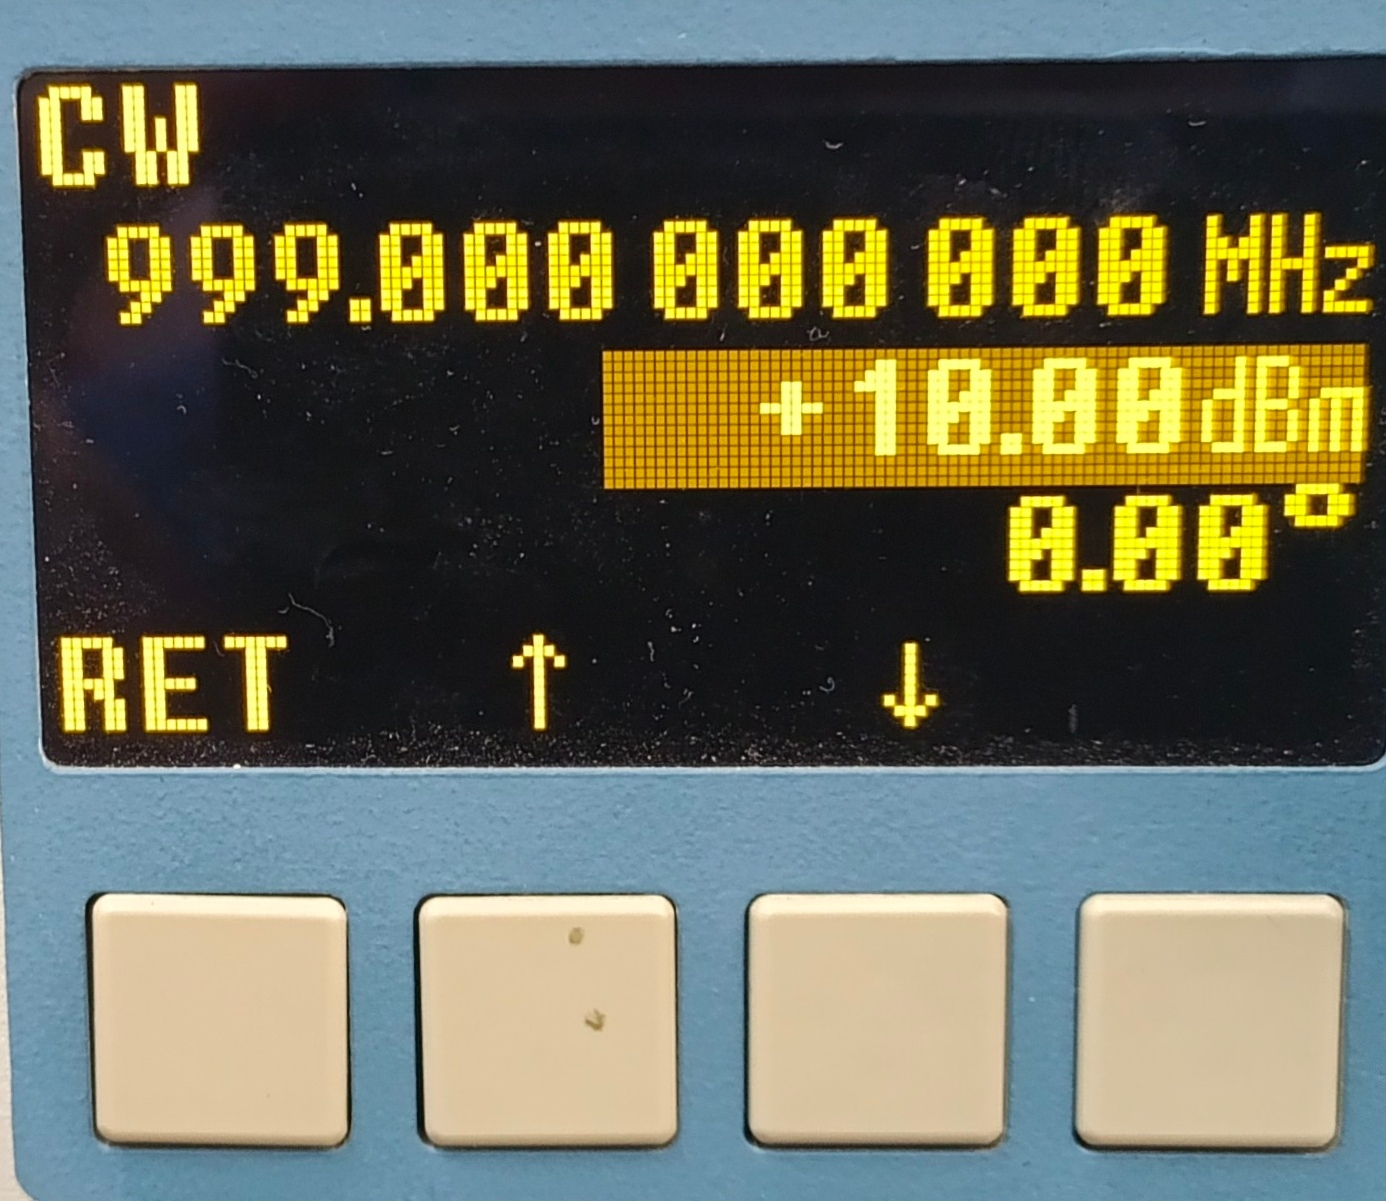
\includegraphics[width=0.48\textwidth]{10дб_3.jpg}
    \caption{Параметры выходного сигнала первого генератора Advantex SG8 ($f_1 = 999\text{ МГц}$, $P_{\text{вых}} = +10\text{ дБм}$)}
    \label{fig:sg_screen}
\end{figure}

\begin{figure}[H]
    \centering
        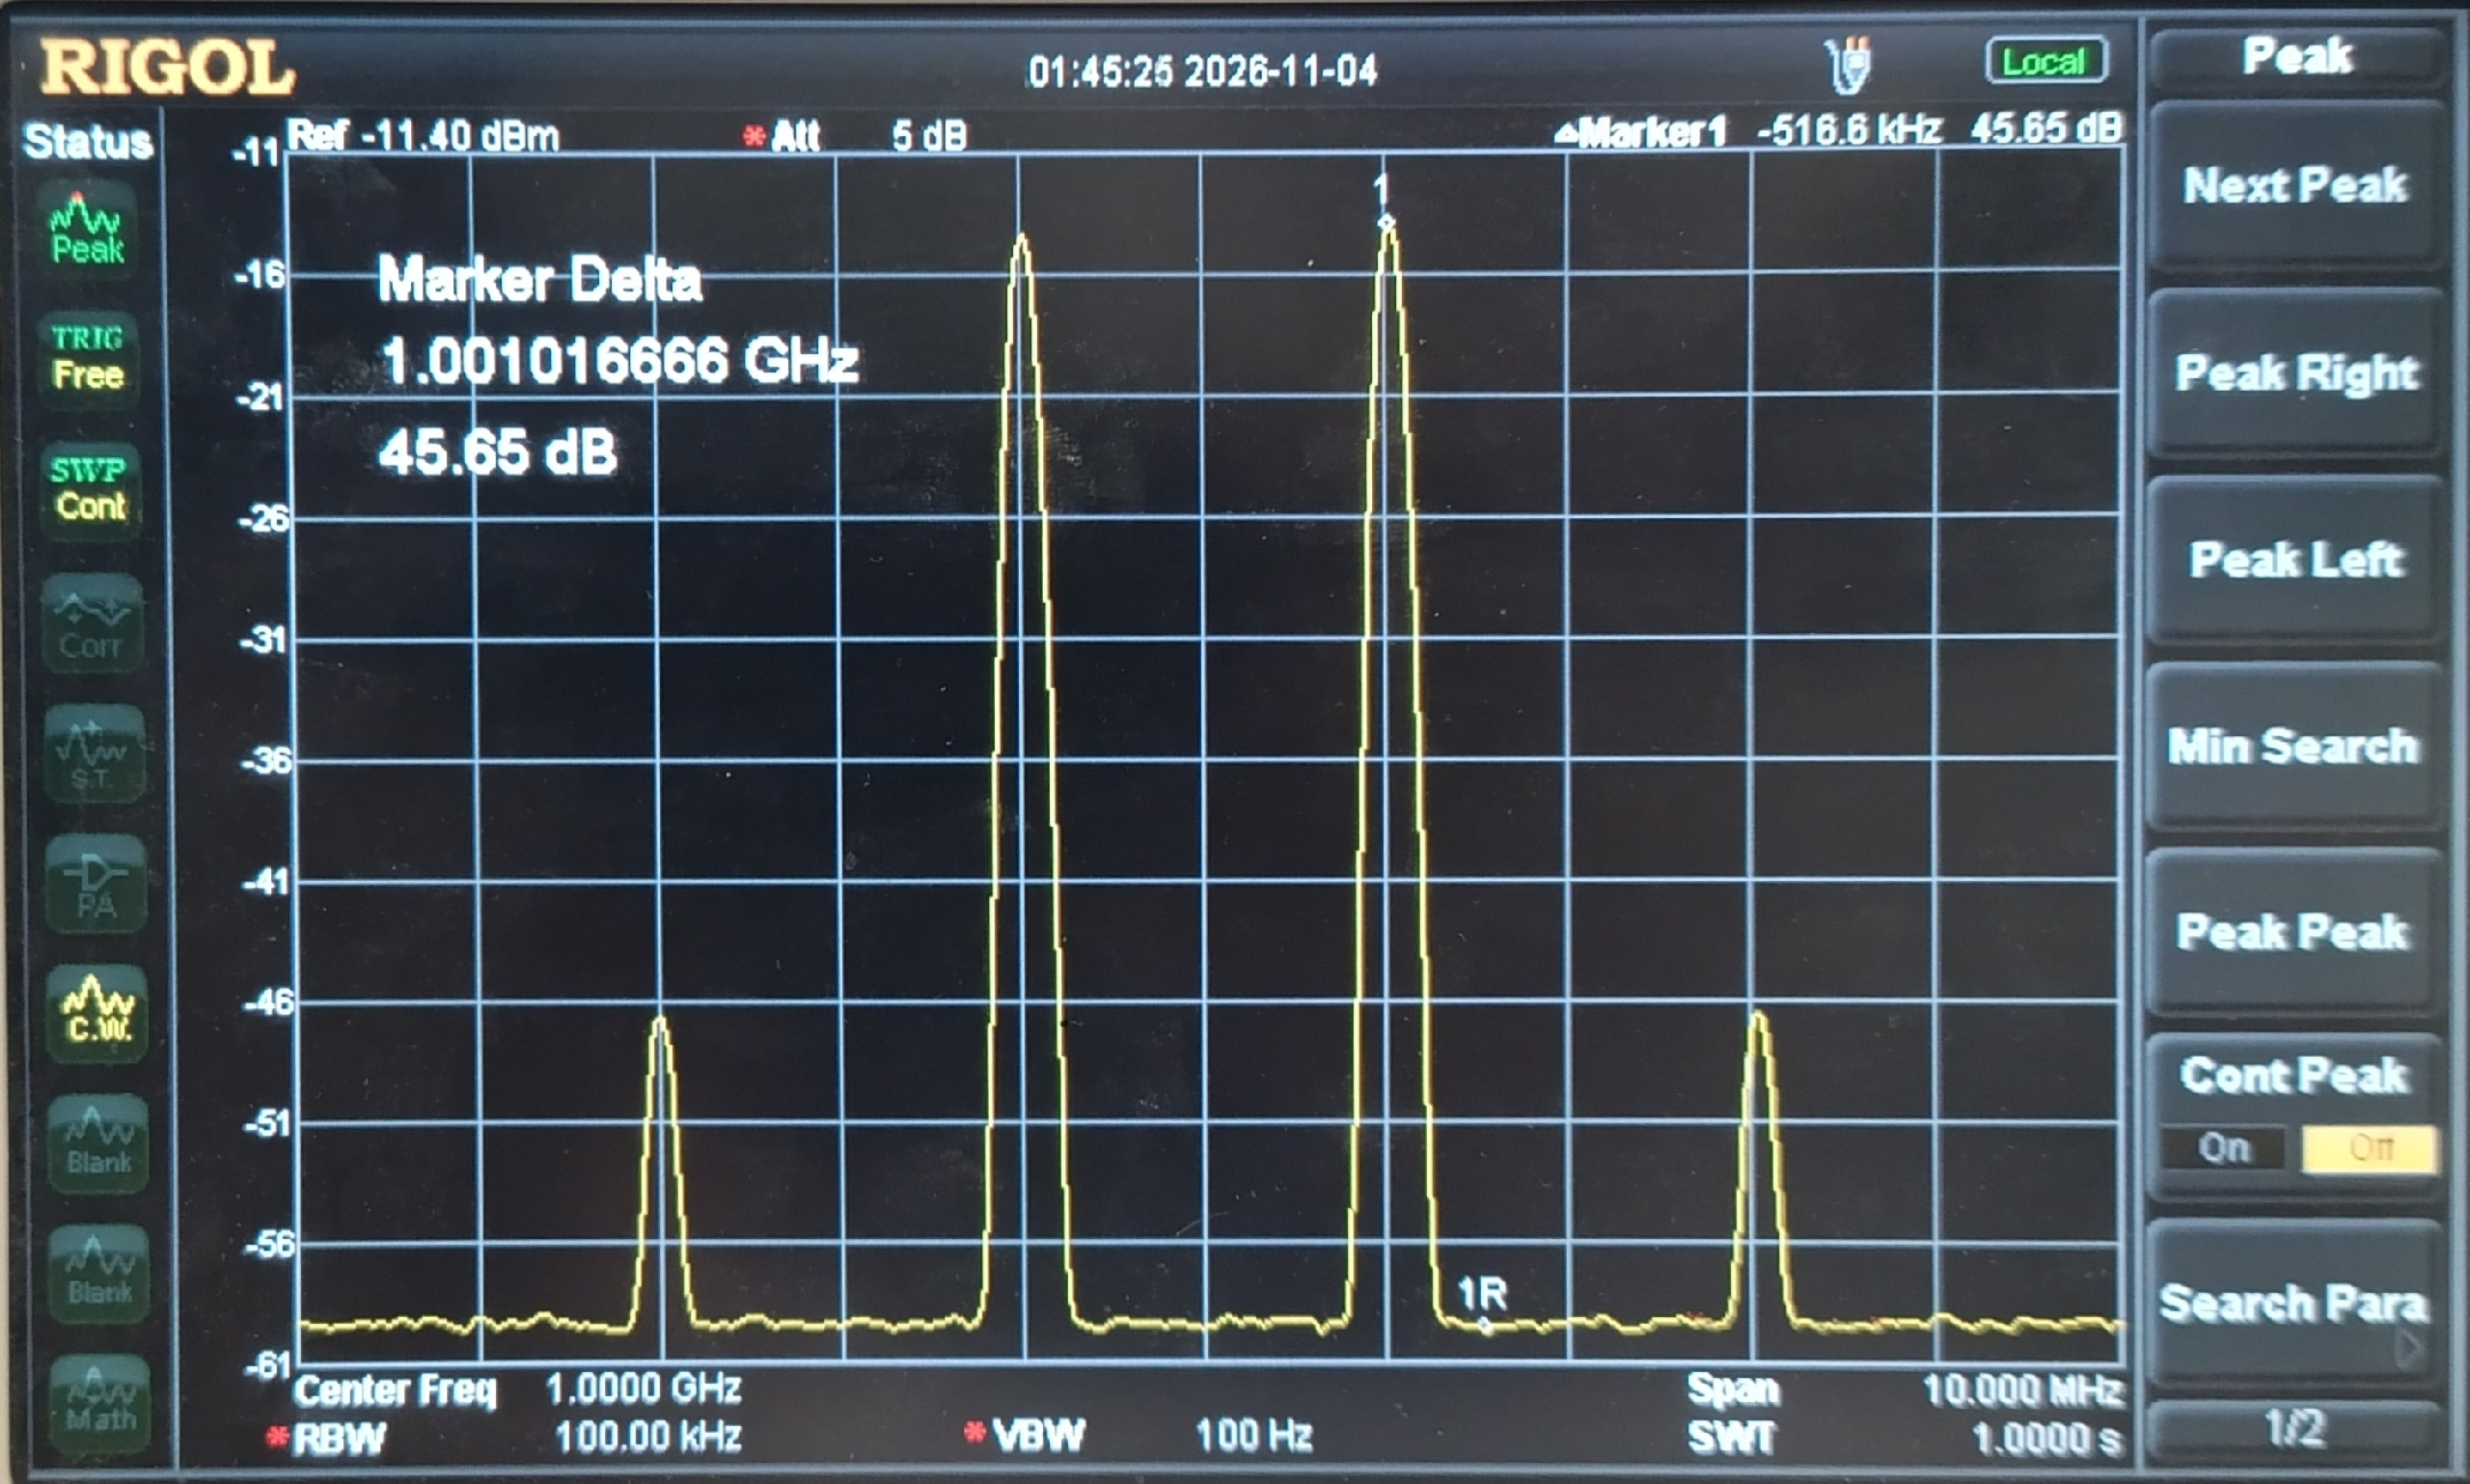
\includegraphics[width=\textwidth]{10дб_2.jpg}
        \caption{Спектрограмма при малом уровне искажений}
        \label{fig:rigol_spec2}
\end{figure}

Результаты измерений уровней гармоник двухтонового сигнала и расчетные значения параметров интермодуляции приведены в таблице~\ref{tab:ip3_data}.

\begin{table}[H]
\centering
\caption{Экспериментальные данные и результаты расчета параметров $IP_3$ ($f_0 = 1\text{ ГГц}$, $\Delta f = 1\text{ МГц}$)}
\label{tab:ip3_data}
\small
\begin{tabular}{|c|c|c|c|c|c|c|}
\hline
$P_{\text{вх}}$, дБм & $P_{f_{1,2}}$, дБм & $IM_3$, дБм & $IMD_3$, дБ & $K_p$, дБ & $OIP_3$, дБм & $IIP_3$, дБм \\
\hline
0  & -20.0 & -59.0 & 39.0 & -20.0 & -0.5 & 19.5 \\
2  & -19.0 & -55.0 & 36.0 & -21.0 & -1.0 & 20.0 \\
4  & -17.0 & -53.0 & 36.0 & -21.0 &  1.0 & 22.0 \\
6  & -15.0 & -47.0 & 32.0 & -21.0 &  1.0 & 22.0 \\
8  & -13.0 & -41.0 & 28.0 & -21.0 &  1.0 & 22.0 \\
10 & -15.0 & -46.0 & 31.0 & -25.0 &  0.5 & 25.5 \\
\hline
\end{tabular}
\end{table}

По результатам эксперимента в среде MATLAB построен график экстраполяции характеристик линейного отклика и продуктов интермодуляции 3-го порядка (рис.~\ref{fig:ip3_matlab}).

\begin{figure}[H]
    \centering
    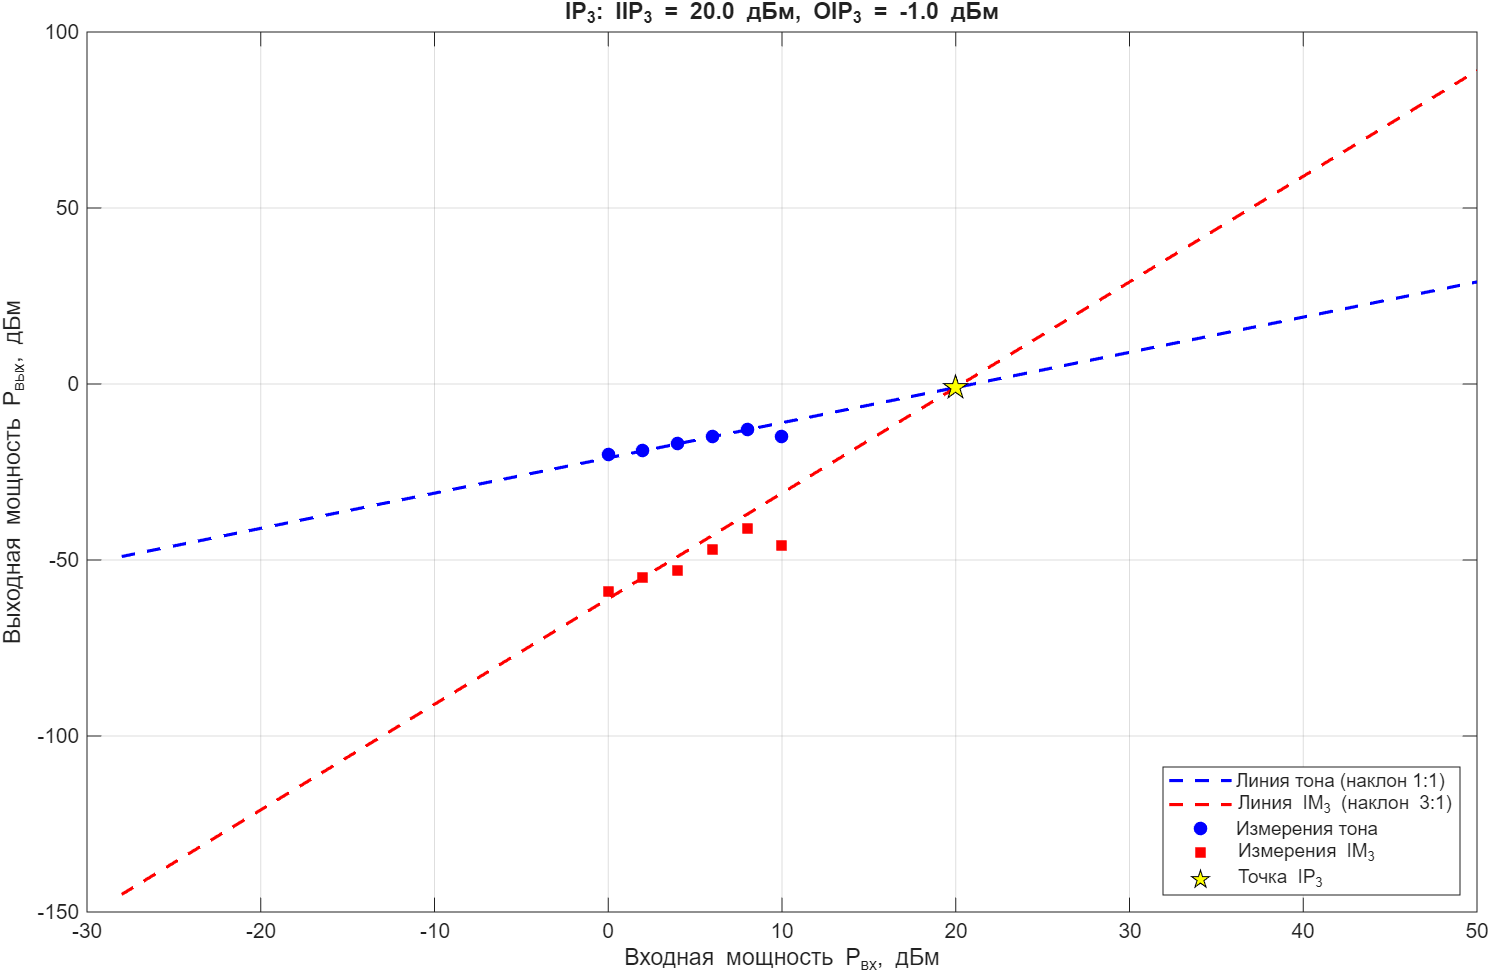
\includegraphics[width=0.88\textwidth]{IP3.png}
    \caption{Графическое определение точки пересечения по интермодуляции третьего порядка ($IP_3$)}
    \label{fig:ip3_matlab}
\end{figure}

По результатам аппроксимации характеристик в малосигнальной области получены следующие координаты точки пересечения третьего порядка:
\begin{equation}
IIP_3 = +20.0\text{ дБм}, \qquad OIP_3 = -1.0\text{ дБм}.
\end{equation}

\subsection{Анализ результатов и выводы}

\begin{enumerate}
    \item \textbf{Закономерность роста интермодуляционных составляющих:} В области малого входного сигнала ($P_{\text{вх}} \le 8\text{ дБм}$) наблюдается строгая теоретическая закономерность нелинейности третьего порядка. При росте входной мощности на 2~дБ мощность полезного тона возрастает на 2~дБ (наклон 1:1), в то время как уровень продуктов интермодуляции $IM_3$ возрастает примерно на 6~дБ (наклон 3:1), вследствие чего параметр $IMD_3$ ухудшается на 4~дБ.
    \item \textbf{Переход в область насыщения:} При значении входной мощности $P_{\text{вх}} = 10\text{ дБм}$ наблюдается спад коэффициента передачи тракта (падение $P_{f_{1,2}}$ до $-15\text{ дБм}$), что свидетельствует о перегрузке каскада и выходе за границы применимости полиномиальной модели слабой нелинейности.
    \item \textbf{Линейность тракта:} Полученное значение точки пересечения $IIP_3 = +20.0\text{ дБм}$ ($OIP_3 = -1.0\text{ дБм}$) существенно превышает уровень точки компрессии $P_{1\text{dB}}$ ($OP_{1\text{dB}} \approx -0.64\text{ дБм}$). Это обеспечивает запас линейности исследуемого тракта и подтверждает малый уровень интермодуляционных искажений при работе в штатном динамическом диапазоне приемника.
\end{enumerate}